\documentclass{article}

% if you need to pass options to natbib, use, e.g.:
% \PassOptionsToPackage{numbers, compress}{natbib}
% before loading nips_2018

% ready for submission
% \usepackage{nips_2018}

% to compile a preprint version, e.g., for submission to arXiv, add
% add the [preprint] option:
% \usepackage[preprint]{nips_2018}

% to compile a camera-ready version, add the [final] option, e.g.:
\usepackage[final]{nips_2018}

% to avoid loading the natbib package, add option nonatbib:
% \usepackage[nonatbib]{nips_2018}

\usepackage[utf8]{inputenc} % allow utf-8 input
\usepackage[T1]{fontenc}    % use 8-bit T1 fonts
\usepackage{hyperref}       % hyperlinks
\usepackage{url}            % simple URL typesetting
\usepackage{booktabs}       % professional-quality tables
\usepackage{amsfonts}       % blackboard math symbols
\usepackage{nicefrac}       % compact symbols for 1/2, etc.
\usepackage{microtype}      % microtypography
\usepackage{graphicx}

\title{Summer2Monsoon: Using CycleGAN for Image-to-Image Translation} 

% The \author macro works with any number of authors. There are two
% commands used to separate the names and addresses of multiple
% authors: \And and \AND.
%
% Using \And between authors leaves it to LaTeX to determine where to
% break the lines. Using \AND forces a line break at that point. So,
% if LaTeX puts 3 of 4 authors names on the first line, and the last
% on the second line, try using \AND instead of \And before the third
% author name.

\author{
  Arnav Garg \\
  Department of Computer Science\\
  UCLA\\
  \texttt{arnavgarg@cs.ucla.edu} \\
  \And
  Simranjit Singh \\
  Department of Computer Science\\
  UCLA\\
  \texttt{simranjit@cs.ucla.edu} \\
   \And
  Tanmay Sardesai \\
  Department of Computer Science\\
  UCLA\\
  \texttt{tanmays@cs.ucla.edu} \\
}

\begin{document}
% \nipsfinalcopy is no longer used

\maketitle

\begin{abstract}
 


\end{abstract}

\section{Introduction}

In the past couple of years, there has been a lot of research done on cross domain image to image translation, where an image is taken from one domain and then transformed into an image of the target domain. This is particularly important as a large number of Computer Vision and Machine Learning problems can viewed as an image-to-image translation problem. For example, noise reduction can be considered a mapping between a noisy image to a corresponding noise free image. For many tasks, it is either very difficult or impossible to find paired data, and so in-order to find a mapping between different domains of images, an un-supervised setting is required. The goal of unsupervised image to image translation is to learn the mapping of special characteristics of one image collection and finding how these characteristics could be translated into the other image collection, all in the absence of any paired training examples.

In this paper, we  perform image-to-image translation using cycle-consistent adversarial network, also known as CycleGAN,  to translate a summer scene into a rainy one and visa versa. We also perform single image de-raining. Some of the applications of this include, helping the film industry shoot movies irrespective of the seasonal cycle and helping self-driving car researchers in data collection by transforming summer images to rainy images, which would allow them to train their models on both these environments simultaneously thereby decreasing the time needed for data collection and training.


%    Experiments on self-driving cars have been conducted since at least the 1920’s [7]
%    and the first truly autonomous cars appeared in the 1980’s, with Carnegie 
%    Mellon University’s Navlab [8]. Waymo, a subsidiary of Alphabet, 
%    began their self driving car project in 2009. Waymo uses deep learning 
%    to interpret, predict and respond to data collected from it’s 6 million 
%    miles driven on public roads and 5 billion driven in simulation [9]. 
%    The way an autonomous car reacts to a situation is hugely dependent on 
%    the weather conditions of the environment it is in. For example, a 
%    self-driving car would drive slower and more cautiously during the 
%    monsoon season than during the summer time due to various environment
%     factors such as lack of visibility and slippery roads. 
%     Training the deep learning model for self-driving cars on 
%     simulations of different weather conditions can be a daunting 
%     task as weather conditions are seasonal and can immensely delay 
%     the time needed for data collection and training.

%We propose a novel method of translating frames/images of environments 
%taken in the summer season to the monsoon season and back. 
%This would allow the data collected by researchers during 
%summer to transform into monsoon conditions and train their 
%models on both these environments simultaneously thereby 
%decreasing the time needed for data collection and training.

%To solve this, we plan to use CycleGAN, which performs image to image 
%translation, by learning the mapping between input image and output image 
%using a training set of unpaired image pairs [1]. CycleGAN captures the 
%special characteristics of one domain and finds out how these 
%characteristics could be translated into the other domain, all in the 
%absence of any paired training examples. In our research, one image 
%collection would be of images taken in during the summer season and 
%the other during the monsoon season. We will discuss this is in greater 
%detail in Section \ref{headings}.  

Some of the other applications of our research include solving the problem of de-raining. There has been various research 
 done on de-raining, as discussed in Section \ref{relatedworks} and we believe that our proposed model would be able to solve the problem by training it to transform rainy images to summer.


% \begin{figure}[htb!]
%  \centering
%  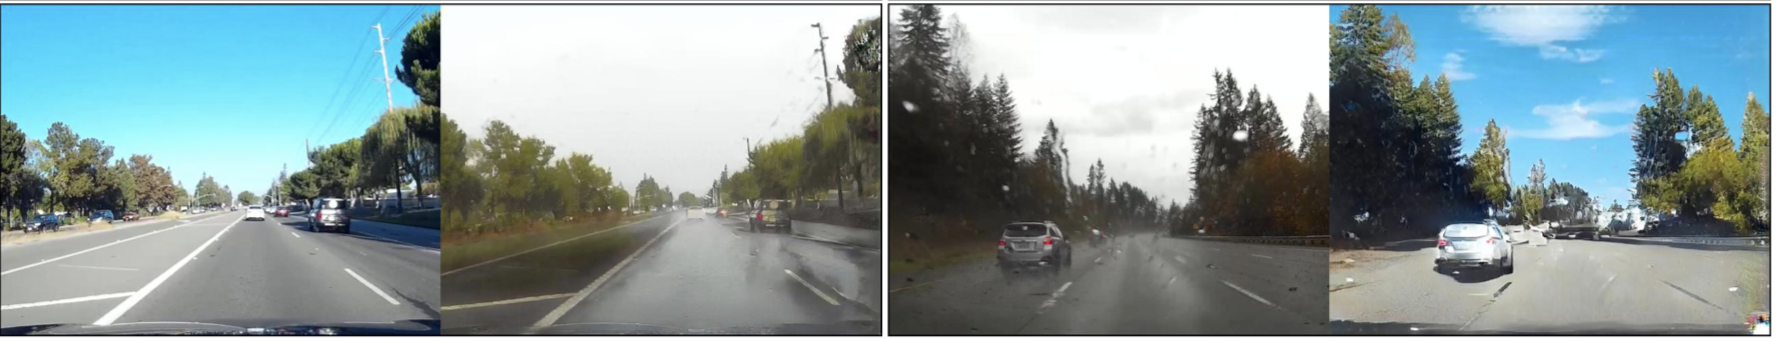
\includegraphics[width=99mm]{image.png}
%  \caption{Taken from nvidia paper. Goal of this project is to do better
%  than this using cycle gan \label{overflow}}
%\end{figure}


\section{Related Work}
\label{relatedworks}

\textbf{Generative Adversarial Networks (GANs)} [2] were introduced by  Ian Goodfellow in 2014 and have been very successful in image-to-image translations. GANs have one neural network that generates data while the other discriminates between real and fake (generated) data. Over time both networks get better at their tasks and the generator is now able to mimic the distribution of the input domain. GAN was used for a variety of applications and it has paved a way for series of GAN-family implementations for different applications.

\textbf{Image-to-Image translation} is the core of this project. The work that we will be exploring in this paper is CycleGAN [1]. Given two domains, $X$ and $Y$, and two generators $G: X \rightarrow Y$ and $F: Y \rightarrow  X$ then we try to achieve a cycle-consistency such that $F(G(X)) \approx X$ and $G(F(Y)) \approx Y$. There is also other work done in the domain of image-to-image translation. The authors of CycleGAN previously proposed pix2pix [5] which used Conditional GANs. pix2pix also has multiple applications but one of the constraints is that pix2pix needs paired data for training. This is sometimes impossible or a really difficult task. For example in our case we would need images taken from the same exact location in 2 different seasons for our dataset. Some related work on image-to-image translation is also done by Nvidia using coupled GAN [3]. Concurrent to the work done in CycleGAN, Yi et al [6], published a paper on dual-GAN.

\textbf{Single Image de-raining} is a difficult problem to solve due to its ill-posed nature and unlike video based methods, images do not provide any temporal information. Traditionally it has been approached as considering an image y to be the sum of rain streak r and background image x, i.e. $y = x + r$. This is why most of the research approaches try to decompose the image into a background image and rain streak image. One of the earliest methods is sparse coding based [a] where image is decomposed using learned dictionary atoms that can sparsely represent two components clearly. Gaussian mixture models based priors [c] have also been used in image decomposition frameworks that can capture different orientations and scales of rain streaks. CNNs have also been employed to directly learn non linear mapping between synthesized images and ground truths successfully for image de-raining [d] [e] [f]. Conditional GANs are also used to achieve de-raining [4]. The work in this, and other papers on de-raining, doesn’t completely solve the problem as they only remove rain from the image but some aspects of the image still look the same as the sky will still look cloudy and the roads will look wet even after removing the rain. These models only work on monsoon to summer translations but not vice versa.

\section{Implementation}

\section{Results}

We performed two different types of studies to help evaluate our results. For our image to image translation, we performed a perceptual study where we created a survey and asked participants to classify if images were real or fake and for the Single Image De-raining, as we had ground truth for these images, we computed the Structural Similarity Index Scores (SSIM) between to de-rained images and the ground-truth to evaluate how well our model performed. We have discussed both of these studies on in the subsection below.

\subsection{Perceptual Study}

\begin{table} [h!]
\centering
\begin{tabular}{ | c | c | c | c |}
\hline
 Type & Total & Real & Fake \\ 
\hline
 Sunny &  0.591 & 0.825 & 0.543 \\  
 Rainy & 0.597 & 0.716 & 0.578 \\
 \hline
\end{tabular}
\caption{Survey Results}
\label{table:1}
\end{table}

For evaluating our image to image translation model, we conducted two online surveys, one with only summer images and the other with rainy images, in which we showed multiple fake (our model generated) and real images to the participant. In both the surveys, the participants were shown each image for 2 seconds, and then were asked to identify if the image they saw was fake or real. The results of the surveys are shown in table \ref{table:1}.

@arnav explain the table

\subsection{SSIM}

@arnav do this

\section{Limitation \& Discussions}



%\section{Research Plan and Expected Outcome (ARCHIVE)}
%\label{headings}
%
%For this project we will train the implementation cycleGAN provided by the 
%authors of [1] on our dataset. Both Pytorch and Torch implementations are 
%available. Our dataset consists of 2 sets of images: summer images and :
%rainy images. There is no one-to-one correspondence between the two sets. 
%We will first search for the image datasets and if we do not find any, we 
%plan to scrape images of summer and rainy season from the web and scale 
%them to same size (say 256 x 256). Since the cycleGAN assumes some 
%underlying relationship between the images from two sets, our first 
%attempt will be to obtain images of the same place corresponding to the 
%two seasons and divide them into train and test datasets. The images can
%be obtained using google or Flickr API for a particular place and 
%categorize into summer vs rainy based on the time of the year the 
%pictures were taken. If the model works well on this dataset, we will 
%attempt to train the model on datasets where the images in each set can 
%be unrelated.
%
%The first obvious expected outcome of our project is that the training 
%error of our model converges and we are able to train the model. In that 
%case, we will evaluate if the model works well on the test dataset and is 
%able to produce images that are able to fool the human eyes. We will also 
%quantitatively evaluate the results. The first measure is the cycle loss 
%that is the difference between the original image and the one obtained 
%after complete cycle. For example, give a test image from the summer 
%dataset, we first convert it to rainy and then back to summer and measure 
%how different it is from the original image. Although this is not a very 
%good measure of what we are trying to achieve because any translation that 
%can be reversed will have a low cycle loss but it definitely is a sanity 
%check for the results.
%
%If our model trains and tests well on images of the same place, we will 
%evaluate the performance of the model on images that may be from different 
%places. We plan to compare our results with existing approaches that solve 
%the problem of image to image translation or image de-raining.
%
%Generative networks are considered much harder to train than discriminative 
%networks. Similarly GANs are difficult to train and require a balance 
%between the discriminator and generator networks for the training loss 
%to converge. GANs are also highly sensitive to hyperparameters. 
%As a part of this project, we also plan to evaluate the impact of 
%hyperparameters on training the cycleGAN network. We aim to study and 
%experiment methods suggested by the authors of CycleGAN to mitigate the 
%model parameters oscillation.

\section{Conclusion \& Future Work}

We have employed the CycleGAN model for the purpose of translating images from summer to monsoon and vice-versa. We were successfully able to train the model to minimize the proposed loss function on our final dataset collected from various sources. We conducted a survey to see if users can identify fake images as real and achieved results comparable to what is discussed in CycleGAN paper. We also employed CycleGAN to de-rain the images as well as add rain to images and evaluated the results based on SSIM scores and compared to some of the previous works.

In future, we want to explore the model used in [3] that involves shared latent space and believe that it would give better results than our current model. In our model the generator loss did not converge but overall loss did and that is something we are keen on analyzing. The loss proposed in CycleGAN is weighted sum of different losses and we believe that these weights can be tuned to achieve even better results.

\section*{References}

\small
\label{[1]}[1] J. Zhu, T. Park, P. Isola, and A. A. Efros. Unpaired image-to-image 
translation using cycle-consistent adversarial networks. 
In International Conference on Computer Vision (ICCV), to appear, 2017

\label{[2]}[2] I. Goodfellow, J. Pouget-Abadie, M. Mirza, B. Xu, D. Warde-Farley, 
S. Ozair, A. Courville, and Y. Ben- gio. Generative adversarial nets. 
In NIPS, 2014.

\label{[3]}[3] M.-Y. Liu, T. Breuel, and J. Kautz. Unsupervised 
image-to-image translation networks. arXiv preprint arXiv:1703.00848, 2017

\label{[4]}[4] H. Zhang, V. A. Sindagi, and V. M. Patel. Image de-raining using a conditional generative 
adversarial network. arXiv preprint arXiv:1701.05957, 2017.

\label{[5]}[5] P. Isola, J.-Y. Zhu, T. Zhou, and A. A. Efros. 
Image-to-image translation with conditional adversarial networks. 
In CVPR, 2017

\label{[6]}[6] Z. Yi, H. Zhang, T. Gong, Tan, and M. Gong. Dualgan: 
Unsupervised dual learning for image-to-image translation. 
In ICCV, 2017

\label{[7]}[7] "'Phantom Auto' will tour city". The Milwaukee Sentinel. 
Google News Archive. 8 December 1926. Retrieved 2013.

\label{[8]}[8] "Carnegie Mellon". Navlab: The Carnegie Mellon University Navigation Laboratory. 
The Robotics Institute. Retrieved 2014.

\label{[9]}[9] Hawkins, Andrew J. “Inside the Lab Where Waymo Is Building 
the Brains for Its Driverless Cars.” The Verge, The Verge, 
www.theverge.com/2018/5/9/17307156/google-waymo-driverless-cars-deep-learning-neural-net-interview, 2018.

\end{document}
